\chapter{Αναγνώριση προσώπων}\label{ch:facerec}

Στο κεφάλαιο αυτό θα μιλήσουμε για τη διαδικασία της αναγνώρισης προσώπου. Η
διαδικασία αυτή διαφέρει από τη διαδικασία της ανίχνευσης προσώπου όσον αφορά τα
εξής:

\begin{description}
  \item[Ανίχνευση Προσώπου] \hfill \\
    Έχει ως σκοπό τον εντοπισμό προσώπων (θέση, διαστάσεις) εντός μιας εικόνας
    και πιθανότητα την εξαγωγή τους για να χρησιμοποιηθούν από τη διαδικασία της
    αναγνώρισης προσώπων

  \item[Αναγνώριση Προσώπου] \hfill \\
    Παραλαμβάνει μια εικόνα προσώπου από την προηγούμενη διαδικασία και έχει ως
    σκοπό είτε \textbf{α)} να ταυτοποιήσει -κάνοντας μία $1x1$ σύγκριση- ότι το
    πρόσωπο αυτό ταυτίζεται με ένα συγκεκριμένο πρόσωπο που δέχθηκε ως είσοδο
    είτε \textbf{β)} να αναγνωρίσει το πρόσωπο πραγματοποιώντας $1xN$ συγκρίσεις
    με ένα σύνολο από εικόνες προσώπων.

\end{description}

Η αναγνώριση προσώπων είναι μια εύκολη διαδικασία για τον ανθρώπινο εγκέφαλο.
Έρευνες \cite{tuchima2006} έχουν δείξει ότι ακόμη και ένα βρέφος τριών ημερών είναι σε
θέση να διακρίνει μεταξύ γνωστών προσώπων.Σύμφωνα με τις
εργασίες των David Hubel\flink{https://en.wikipedia.org/wiki/David_H._Hubel}
και Torsten Wiesel\flink{https://en.wikipedia.org/wiki/Torsten_Wiesel}  ο ανθρώπινος εγκέφαλος έχει εξειδικευμένους
νευρώνες οι οποίοι ανταποκρίνονται σε συγκεκριμένα χαρακτηριστικά μιας οπτικής
εικόνας -όπως οι γραμμές, οι ακμές, οι γωνίες και η κίνηση- και τα οποία
επεξεργάζεται καταλλήλως και δημιουργεί πρότυπα. Πάνω σε αυτό το πλαίσιο λειτουργεί
και η αναγνώριση προσώπων από υπολογιστές, στην εξαγωγή συγκεκριμένων χαρακτηριστικών
από μια εικόνα, την αναπαράστασή τους με μια αναγνωρίσιμη από υπολογιστές μορφή
και τη διενέργεια κάποιου είδους ταξινόμησης μέσα από αυτά.


Η πιο συνήθης προσέγγιση είναι η αναγνώριση προσώπων χρησιμοποιώντας κάποια
γεωμετρικά χαρακτηριστικά του προσώπου. Μια πρώτη προσέγγιση πάνω στο προαναφερθείσα
λογική περιγράφεται εδώ \cite{Kanade-1973-15078} όπου χαρακτηριστικά όπως τα μάτια, η μύτη, τα
αυτιά κ.α. χρησιμοποιούνται για την κατασκευή διανυσμάτων σχετικά με τη θέση,
την απόσταση και τη γωνίας μεταξύ τους. Στη συνέχεια υπολογίζεται η ευκλείδεια
απόσταση μεταξύ των προηγουμένως υπολογισμένων διανυσμάτων και των διανυσμάτων
μιας εικόνας με ένα γνωστό πρόσωπο. Συγκρίνοντας τις αποστάσεις με διάφορα δείγματα
το πρόσωπο που αναγνωρίζεται θεωρείται το δείγμα με την μικρότερη απόσταση. Παρόλο
που η μέθοδος αυτή δεν επηρεάζεται από τις αλλαγές στο φωτισμό, σύμφωνα με
μελέτες \cite{Brunelli:1992:FRT:645305.648740}, τα γεωμετρικά χαρακτηριστικά ενός προσώπου δεν παρέχουν αρκετή πληροφορία
για ακριβή αποτελέσματα.

Κατά καιρούς διάφορες μέθοδοι έχουν προταθεί. Οι πιο χαρακτηριστικές είναι:

\begin{enumerate}
  \item \emph{EigenFaces - 1991 ~\cite{Turk:1991:ER:1326887.1326894}}
  \item \emph{Local Binary Patterns Histograms - 1996 ~\cite{10.1007/978-3-540-24670-1_36}}
  \item \emph{FisherFaces - 1997 ~\cite{behekri97}}
  \item \emph{Scale Invariant Feature Transform (SIFT) - 1999 ~\cite{790410}}
  \item \emph{Speed Up Robust Features (SURF) - 2006 ~\cite{BAY2008346}}
\end{enumerate}

Οι μέθοδοι EigenFaces και FisherFaces, όπως και οι SIFT και SURF χρησιμοποιούν
τις ίδιες τεχνικές για την εξαγωγή των χαρακτηριστικών μιας εικόνας και τη σύγκρισή
τους με το σύνολο των εικόνων που δέχτηκαν ως είσοδο.

Παρακάτω θα δοθεί μια περιγραφή για τις τρεις πρώτες μεθόδους και να αναλυθεί
το σημείο της μεθόδου LBPH που τροποποιήθηκε στα πλαίσια αυτής της διπλωματικής.


\section{H μέθοδος EigenFaces}\label{sec:eigen}

Το πρόβλημα με την αναπαράσταση εικόνας που χρησιμοποιείται είναι ότι αναπαρίσταται
στο διανυσματικό χώρο με ένα διάνυσμα πολλών διαστάσεων. Για παράδειγμα μια ασπρόμαυρη
εικόνα δύο (2) διαστάσεων $p x q$ αναπαρίσταται με ένα διάνυσμα $m=pq$-θέσεων.
Οπότε μια εικόνα $100 x 100$ pixels παράγει ένα διάνυσμα $10,000$ θέσεων.
Στην πραγματικότητα όμως για να εξάγουμε συμπεράσματα στο εν λόγω πρόβλημα της
αναγνώρισης προσώπων δε μας είναι απαραίτητη το σύνολο της πληροφορίας που υπάρχει
σε ολόκληρη την εικόνα. Χρειάζεται να εντοπίσουμε τις υποπεριοχές της
εικόνας οι οποίες περιέχουν την πληροφορία που χρειαζόμαστε για την αναγνώριση
του προσώπου. Η βασική ιδέα για να επιλέξουμε την πληροφορία που χρειαζόμαστε είναι
ότι ένα διάνυσμα πολλών διαστάσεων συνήθως περιγράφεται από ένα σύνολο μεταβλητών
που συσχετίζονται μεταξύ τους και επομένως χρειάζονται μόνο ορισμένες για να εξαχθεί
η πληροφορία που χρειαζόμαστε. Η παραπάνω ιδέα αναλύεται στη μέθοδο
Principal Component Analysis (PCA) η οποία προτάθηκε τόσο από τον Karl Pearson
\flink{https://en.wikipedia.org/wiki/Karl_Pearson} (1901) όσο και από τον
Harold Hotelling \flink{https://en.wikipedia.org/wiki/Harold_Hotelling} (1933) και περιγράφει
πως ένα σύνολο πιθανώς συσχετιζόμενων μεταβλητών περιγράφεται επαρκώς από ένα
μικρότερο σύνολο μη-συσχετιζόμενων μεταβλητών.

\subsection{Περιγραφή του αλγορίθμου}\label{subsec:eigenalgo}

Έστω $X = \{x_1, x_2, ..., x_n\}$ ένα τυχαίο διάνυσμα όπου κάθε $x_i \in \mathbb{R}^d$

\begin{enumerate}
    \item Υπολόγισε τον μέσο $\mu$
        \begin{equation}
            \mu = \frac{1}{n}\sum_{i=1}^{n} x_i
            \tag{1}
        \end{equation}

    \item Υπολόγισε την μήτρα συνδιακύμανσης $S$
        \begin{equation}
            S = \frac{1}{n}\sum_{i=1}^{n} (x_i-\mu)(x_i-\mu)^T
            \tag{2}
        \end{equation}

    \item Υπολόγισε τις ιδιοτιμές (eigenvalues) $ \lambda_i $ και τα ιδιοδιανύσματα (eigenvectors) $ v_i $
        \begin{equation}
            Sv_i = \lambda_i v_i
            \tag{3}
        \end{equation}

    \item Ταξινόμησε τα ιδιοδιανύσματα σε φθίνουσα σειρά σύμφωνα με τις ιδιοτιμές τους. Τα $ k $ κυριότερα στοιχεία
        είναι τα ιδιοδιανύσματα που αντιστοιχούν στις $ k $ μεγαλύτερες ιδιοτιμές.
\end{enumerate}

Τα $ k $ κυριότερα στοιχεία του διανύσματος $ x $ δίνονται από τον ακόλουθο τύπο
\begin{equation}
    y = W^T(x-\mu)
    \tag{4}
    \label{eq:4}
\end{equation}όπου
$ W = (v_1, v_2, \ldots, v_k) $
\\
Η ανακατασκευή του διανύσματα χρησιμοποιώντας τη μέθοδο PCA προκύπτει
\begin{equation}
    x = Wy + \mu
    \tag{5}
    \label{eq:5}
\end{equation}

Η αναγνώριση του προσώπου με τη μέθοδο Eigenface γίνεται με τον εξής τρόπο:
\begin{enumerate}
    \item Αρχικά αναπαριστούμε με τη μέθοδο PCA όλες τις εικόνες που χρησιμοποιούμε ως δείγματα
        χρησιμοποιώντας την εξίσωση \ref{eq:4}
    \item Αναπαριστούμε με την μέθοδο PCA την προς αναγνώριση εικόνα με βάση την εξίσωση \ref{eq:5}
    \item Συγκρίνουμε την προηγούμενη αναπαράσταση με τις αναπαραστάσεις των δειγμάτων και
        υπολογίζουμε τον κοντινότερο γείτονα
\end{enumerate}

Από πλευράς πολυπλοκότητας, η μέθοδος που ακολουθήσαμε εμπεριέχει ένα πρόβλημα
υπολογιστικού χώρου Ας υποθέσουμε ότι μας δίνονται ως δείγματα 400 εικόνες
μεγέθους 100 x 100 pixels. Ακολουθώντας τη μέθοδο PCA, πρέπει να υπολογίσουμε
τη μήτρα συνδιακύμανσης $ S = XX^T $, όπου \emph{Θ(X)} = 10000 x 400. Καταλήγουμε
με αυτόν τον τρόπο με έναν πίνακα 10000 x 10000, ο οποίος καταλαμβάνει χώρο περίπου
\emph{0.8GB}.
Προκειμένου να μειώσουμε αυτό το χώρο, μπορούμε να χρησιμοποιήσουμε από τη γραμμική
άλγεβρα τη θέση ότι ένας πίνακας $M x N$ όπου $Μ > Ν$ μπορεί να έχει μόνο $N-1$
μη μηδενικές ιδιοτιμές. Επομένως χρησιμοποιώντας την ιδιοαποσύνθεση του $S$, $S=X^TX$
μεγέθους $NxN$ έχουμε:
\begin{equation}
    X^TXv_i = \mu_iv_i
    \tag{6}
    \label{eq:6}
\end{equation}

και από εκεί υπολογίζουμε τα ιδιοδιανύσματα $S = XX^T$ κάνοντας αριστερό πολλαπλασιασμό
πινάκων:
\begin{equation}
    XX^T(Xv_i) = \mu_i(Xv_i)
    \tag{7}
    \label{eq:7}
\end{equation}

Από τα παραγόμενα ορθογώνια ιδιοδιανύσματα, υπολογίζουμε τα αντίστοιχα ορθοκανονικά.

Τα EigenFaces οπτικοποιούνται ακολούθως:



\begin{figure}[htbp]
  \begin{center}
    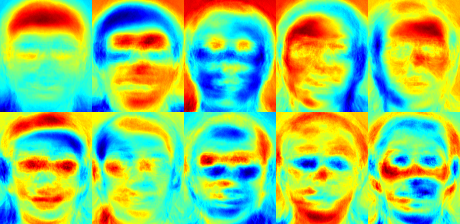
\includegraphics[width=0.8\maxwidth]{../figures/eigenfaces.png}
      \caption{EigenFaces για 10 πρόσωπα της βάσης δεδομένων AT \& T Facedatabase}\footnote{http://www.cl.cam.ac.uk/research/dtg/attarchive/facedatabase.html}
      \label{fig:eigenfaces}
   \end{center}
\end{figure}


\section{H μέθοδος FisherFaces}\label{sec:fisher}

Μία άλλη μέθοδος για τον περιορισμό της επεξεργάσιμης πληροφορία μέσα από μια
εικόνα είναι η μέθοδος FisherFaces. Η μέθοδος αυτή στηρίζεται στη γραμμική
διακριτή ανάλυση (Linear Discriminant Analysis) για τον περιορισμό των διαστάσεων
μιας εικόνας και  προτάθηκε από τον Sir R. A. Fisher
\flink{https://en.wikipedia.org/wiki/Ronald_Fisher}. Ο Fisher
,το 1936, ταξινόμησε με επιτυχία τα \emph{λουλούδια} ως κλάση αντικειμένου.
Το αρνητικό της μεθόδου PCA είναι ότι είναι ευάλωτη σε εξωτερικές πηγές. Πιο
συγκεκριμένα, η μέθοδος PCA βρίσκει έναν γραμμικό συνδυασμό χαρακτηριστικών
της εικόνας ο οποίος μεγιστοποιεί τη διακύμανση ωφέλιμης πληροφορίας. Ο τρόπος
αυτός ενώ μας παρέχει έναν ισχυρό τρόπο αναπαράστασης της πληροφορίας, δεν λαμβάνει
υπ' όψιν την κλάση του αντικειμένου με αποτέλεσμα διακεκριμένη πληροφορία που αφορά
τη συγκεκριμένη κλάση αντικειμένου να χάνεται κατά τη μέθοδο. Ας υποθέσουμε ότι
εισάγεται θόρυβος στην πληροφορία της εικόνας από εξωτερικό φως. Τα στοιχεία που
αναγνωρίζονται από την ανάλυση PCA δεν περιέχουν απαραίτητα κάποια συγκεκριμένη
πληροφορία σχετικά με το θόρυβο από το μια εξωτερική πηγή φωτός. Αυτό καθιστά
την ταξινόμηση του προσώπου αδύνατη.
Η μέθοδος της Linear Discriminant Analysis εστιάζει στην ανεύρεση των χαρακτηριστικών
εκείνων που εντοπίζουν καλύτερα τις διαφορές μεταξύ διάφορων κλάσεων αντικειμένων.
Η ιδέα βασίζεται στο ότι όμοιες κλάσεις ομαδοποιούνται κοντά ενώ διαφορετικές κλάσεις
έχουν απόσταση μεταξύ τους.


\subsection{Περιγραφή του αλγορίθμου}\label{subsec:fisheralgo}

Έστω $X$ τυχαίο διάνυσμα με δείγματα από $C$ κλάσεις:
$$
X = \{X_1,X_2,\ldots,X_c\}
$$
$$
X_i = \{x_1,x_2,\ldots,x_n\}
$$

Οι διεσπαρμένοι πίνακες $S_B$ και $S_W$ υπολογίζονται ως εξής:
$$
S_B = \sum_{i=1}^{c} N_i(\mu_i-\mu)(\mu_i-\mu)^{T}
$$
$$
S_W = \sum_{i=1}^{c} \sum_{x_j \in X_i}^{} (x_j-\mu_i)(x_j-\mu_i)^{T}
$$

όπου $\mu$ είναι ο συνολικός μέσος
$$
\mu = \frac{1}{N}\sum_{i=1}^{N} x_i
$$
και $\mu_i$ είναι ο μέσος της κλάσης $i \in \{1,\ldots,c\}$
$$
\mu_i = \frac{1}{|X_i|}\sum_{x_j \in X_i} x_j
$$
Ο κλασικός αλγόριθμος του Fisher υπολογίζει την προβολή $W$ η οποία μεγιστοποιεί
το κριτήριο διαχωριστικότητας των κλάσεων ως:
$$
W_opt = \operatorname{arg\,max}_W \frac{|W^T S_B W|}{|W^T S_W W|}
$$

Μια λύση για αυτό το πρόβλημα βελτιστοποίησης δίνεται από το γενικότερο Eigenvalue
Problem ~\cite{behekri97}
$$
S_{B}v_i = \lambda_{i}S_{w}v_i
$$
$$
S_{W}^{-1}S_{B}v_i = \lambda_{i}v_i
$$

Τα FisherFaces οπτικοποιούνται ακολούθως:


\begin{figure}[htbp]
  \begin{center}
    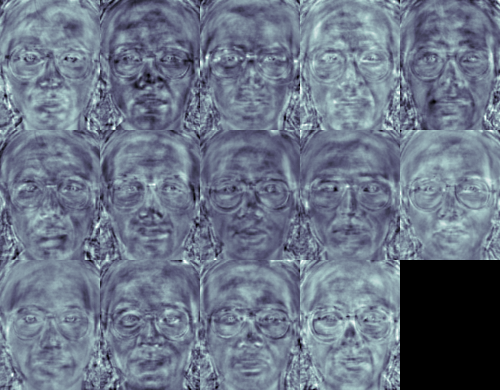
\includegraphics[width=0.5\maxwidth]{../figures/fisherfaces.png}
      \caption{FisherFaces για 16 πρόσωπα της βάσης δεδομένων Yale Facedatabase A}\flink{http://vision.ucsd.edu/content/yale-face-database}
      \label{fig:fisherfaces}
   \end{center}
\end{figure}

Στο σημείο αυτό αξίζει να σημειώσουμε ότι η μέθοδος FisherFace επικεντρώνει στην
επισήμανση των διαφορών μεταξύ των προσώπων και συνεπώς είναι ευαίσθητη στις μεταβολές
του φωτισμού. Ένα σύστημα αναγνώρισης με τη μέθοδο FisherFace εκπαιδευμένο με πρόσωπα
εκτεθειμένα σε έντονο φωτισμό δυσκολεύεται να αναγνωρίσει πρόσωπα σε χαμηλό φωτισμό.
Επομένως, η ποιότητα των αποτελεσμάτων της μεθόδου εξαρτάται σε πολύ μεγάλο βαθμό
από τα δεδομένα (πρόσωπα) εισόδου με τα οποία εκπαιδεύεται ο αλγόριθμος.


\section{H μέθοδος Local Binary Patterns Histograms (LBPH)}\label{sec:lbph}

Η ιδέα πίσω από τη μέθοδο LBPH έγκειται στην εξαγωγή κάποιον τοπικών χαρακτηριστικών
από την εικόνα. Με αυτό τον τρόπο αποφεύγεται η αντιμετώπιση της εικόνας ως ένας πίνακα πολλών
διαστάσεων. Παράλληλα το γεγονός ότι βασίζεται στην ανάλυση υφής (texture analysis)
της εικόνας την καθιστά ανθεκτική σε αλλαγές στην φωτεινότητα, το μέγεθος και την
γωνία (περιστροφή) της εικόνας.

Πιο συγκεκριμένα, τα Local Binary Patterns εφαρμόζονται στην αναπαράσταση της εικόνας
στην κλίμακα grayscale. Υπολογίζουν μια νέα της αναπαράσταση συγκρίνοντας την ένταση
κάθε εικονοστοιχείου (pixel) με αυτή των γειτονικών του. Στην καινούργια αναπαράσταση
τα γειτονικά pixel λαμβάνουν την τιμή $1$ ή $0$ ανάλογα με το αν η ένταση τους είναι
μεγαλύτερη ή μικρότερη από το κεντρικό. Τελικά η τιμή του κεντρικού pixel υπολογίζεται
από την δεκαδική αναπαράσταση της παράθεσης των τιμών των γειτονικών pixel. Η διαδικασία
αυτή επαναλαμβάνεται για όλα τα pixel της εικόνας.\newline
\\
Υπολογισμός Local Binary Pattern:
$$
LBP(x_c, y_c) = \sum_{p=0}^{p-1}2^ps(i_p-i_c)
$$
όπου

$$ s(x) =
  \begin{cases}
    1       & \quad \text{if } x \geq 0\\
    0       & \quad \text{else}
  \end{cases}
$$

Ας δούμε τη μέθοδο με περισσότερη ακρίβεια.\\
\\
Οι βασικές παράμετροι του αλγορίθμου είναι οι εξής:

\begin{description}
    \item[Radius (ακτίνα)] \hfill \\
    Έχει ως σκοπό τον εντοπισμό προσώπων (θέση, διαστάσεις) εντός μιας εικόνας
    και πιθανότητα την εξαγωγή τους για να χρησιμοποιηθούν από τη διαδικασία της
    αναγνώρισης προσώπων. Στην τυπική υλοποίηση της μεθόδου η τιμή \textbf{Radius} είναι $1$.
    \item[Neighbors (πλήθος γειτόνων)] \hfill \\
    Παραλαμβάνει μια εικόνα προσώπου από την προηγούμενη διαδικασία και έχει ως
    σκοπό είτε \textbf{α)} να ταυτοποιήσει -κάνοντας μία $1x1$ σύγκριση- ότι το
    πρόσωπο αυτό ταυτίζεται με ένα συγκεκριμένο πρόσωπο που δέχθηκε ως είσοδο
    είτε \textbf{β)} να αναγνωρίσει το πρόσωπο πραγματοποιώντας $1xN$ συγκρίσεις
    με ένα σύνολο από εικόνες προσώπων. Στην τυπική υλοποίηση της μεθόδου η τιμή \textbf{Neighbors} είναι $8$.
    \item[Grid X] \hfill \\
    Ο αριθμός των οριζόντιων κελιών στον οποίο θα χωριστεί η εικόνα. Όσα περισσότερα
    κελιά έχουμε τόσο μεγαλύτερη είναι η διάσταση του χάρτη χαρακτηριστικών της εικόνας.
    Στην τυπική υλοποίηση της μεθόδου η τιμή \textbf{Grid X} είναι $8$.
    \item[Grid Y] \hfill \\
    Ο αριθμός των κάθετων κελιών στον οποίο θα χωριστεί η εικόνα. Όσα περισσότερα
    κελιά έχουμε τόσο μεγαλύτερη είναι η διάσταση του χάρτη χαρακτηριστικών της εικόνας.
    Στην τυπική υλοποίηση της μεθόδου η τιμή \textbf{Grid Y} είναι $8$.
\end{description}

Χρησιμοποιώντας τις προκαθορισμένες τιμές για την ακτίνα και τους γείτονες έχουμε:


\begin{figure}[htbp]
  \begin{center}
    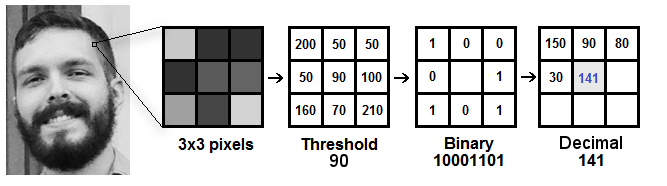
\includegraphics[width=1.0\maxwidth]{../figures/lbph1.png}
    \caption{Υπολογισμός των Local Binary Patterns}
    \label{fig:lbph1}
  \end{center}
\end{figure}

Το αποτέλεσμα είναι μια εικόνα που εμφανίζει σαφέστερα τα χαρακτηριστικά της αρχικής
εικόνας.


\begin{figure}[htp]
    \centering
    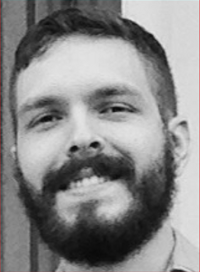
\includegraphics[width=.20\textwidth]{../figures/lbph4.png}\hspace{50pt}%\hfill
    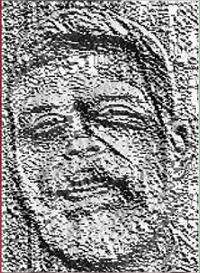
\includegraphics[width=.20\textwidth]{../figures/lbph3.png}\hfill

    \caption{α) αρχική εικόνα σε grayscale, β) ύστερα από το μετασχηματισμό LBP }
    \label{fig:lbph2}

\end{figure}

Στη συνέχεια χρησιμοποιώντας τις παραμέτρους \textbf{Grid X} και \textbf{Grid Y}
η νέα εικόνα χωρίζεται σε ένα πλέγμα διαστάσεων (\textbf{Grid X} $*$ \textbf{Grid Y}).

\begin{figure}[htp]
    \centering
    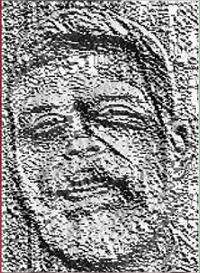
\includegraphics[width=.20\textwidth]{../figures/lbph3.png}\hspace{50pt}%\hfill
    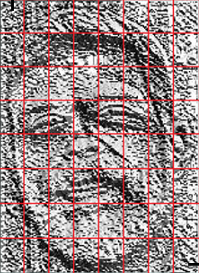
\includegraphics[width=.20\textwidth]{../figures/lbph5.png}\hfill

    \caption{Εξαγωγή ιστογραμμάτων από κάθε υποπεριοχή του πλέγματος}
    \label{fig:lbph3}

\end{figure}

Υπολογίζεται το ιστόγραμμα (histogram) κάθε υποπεριοχής που προκύπτει. Εφόσον η
αρχική εικόνα ήταν σε ασπρόμαυρη κλίμακα (grayscale) το κάθε παραγόμενο ιστόγραμμα
θα περιέχει $256$ θέσεις ($0-255$). Εν τέλει συνθέτουμε όλα τα παραγόμενα ιστογράμματα
σε ένα συνολικό το οποίο αναπαριστά τα χαρακτηριστικά της αρχικής εικόνας. Το τελικό
ιστόγραμμα θα περιέχει (\textbf{Grid X} $*$ \textbf{Grid Y} $*$ $256$ θέσεις).
\paragraph{} \hspace{0em} \\
Ανάλογα με την τιμή των παραμέτρων \textbf{Radius} και \textbf{Neighbors} τα pixel
που συμμετέχουν στον υπολογισμό του Local Binary Pattern αλλάζουν. Για παράδειγμα:
\begin{figure}[htbp]
  \begin{center}
    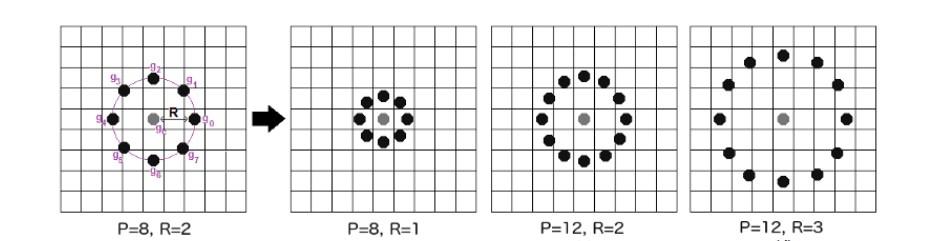
\includegraphics[width=0.8\maxwidth]{../figures/elbp.png}
      \caption{Extended Local Binary Patterns}
      \label{fig:elbp}
   \end{center}
\end{figure}

O νέος αυτός τελεστής , οποίος διαφοροποιείται από το κλασσικό LBP, ονομάζεται
Extended Local Binary Patterns.

\subsection{Τυπική υλοποίηση}\label{subsec:lbphdef}

Στην τυπική υλοποίηση της μεθόδου LBPH, αρχικά κατασκευάζεται μια βάση από ιστογράμματα
από ένα προκαθορισμένο σύνολο εικόνων (training dataset) το οποίο αποτελεί τη βάση
αλήθειας της μεθόδου (ground truth). Για κάθε εικόνα στην οποία θέλουμε να αναγνωρίσουμε ένα
πρόσωπο υπολογίζεται το αντίστοιχο ιστόγραμμα και στη συνέχεια με χρήση του αλγορίθμου
1-Nearest Neighbor \flink{https://en.wikipedia.org/wiki/K-nearest_neighbors_algorithm\#The_1-nearest_neighbor_classifier}
ανιχνεύεται η κλάση (πρόσωπο) καθώς και η ελάχιστη απόσταση μεταξύ των
ιστογραμμάτων της αρχικής εικόνας και της κλάσης. Η εικόνα της κλάσης από την οποία
προκύπτει η ελάχιστη διαφορά επιστρέφεται επίσης ως ένα μέτρο της αξιοπιστίας του αποτελέσματος.
\paragraph{} \hspace{0em} \\
Για να υπολογιστεί η απόσταση δύο ιστογραμμάτων μπορούν να χρησιμοποιηθούν
διάφορα είδη αποστάσεων όπως \texttt{Ευκλείδεια απόσταση}, \texttt{Chi-Square},
\texttt{Απόλυτη τιμή}. Στην τυπική υλοποίηση χρησιμοποιείται η \texttt{Ευκλείδεια απόσταση}.
$$
D = \sqrt{\sum_{i=1}^{n}(hist1_i - hist2_i)^2}
$$

\subsection{Υλοποίηση με τη χρήση του αλγορίθμου k-Nearest Neighbor}\label{subsec:lbphknn}

Στη δικιά μας υλοποίηση, αντικαταστήσαμε των αλγόριθμο προσδιορισμού του προσώπου (1-Nearest Neighbor)
με τον αλγόριθμο k-Nearest Neighbor \flink{https://en.wikipedia.org/wiki/K-nearest_neighbors_algorithm}.
H διαφορά των δύο μεθόδων βρίσκεται στον αριθμό των κοντινών δειγμάτων που θα χρησιμοποιηθούν
\begin{figure}[htbp]
  \begin{center}
    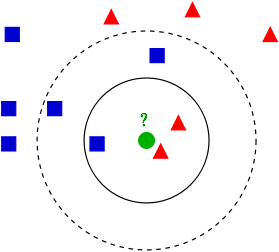
\includegraphics[width=0.8\maxwidth]{../figures/knn.png}
      \caption{Η διαφορά μεταξύ 1-Nearest Neighbor και k-Nearest Neighbor}
      \label{fig:knn}
   \end{center}
\end{figure}

για τον προσδιορισμό της κλάσης Όπως βλέπουμε στο σχήμα \ref{fig:knn} για $k=1$
η κλάση που επιστρέφεται από τον αλγόριθμο είναι η 'κόκκινη' δηλαδή ουσιαστικά
είναι η κλάση που βρίσκεται στην μικρότερη απόσταση από το δείγμα. Για $k=3$ η κλάση
που υπολογίζεται είναι και πάλι η 'κόκκινη' καθώς λαμβάνοντας υπόψιν τα 3 κοντινότερα
σημεία στο δείγμα μας παρατηρούμε ότι τα 'κόκκινα' είναι περισσότερα από τα 'μπλε'.
Όμως για $k=5$ παρατηρούμε ότι τα 'μπλε' είναι περισσότερα από τα 'κόκκινα' οπότε
σε αυτή την περίπτωση τη κλάση που επιστρέφει ο αλγόριθμος ταξινόμησης είναι η 'μπλε'.
\paragraph{} \hspace{0em} \\
Στο επόμενο κεφάλαιο θα αναλύσουμε με σαφήνεια τα αποτελέσματα της χρήσης του
αλγορίθμου k-Nearest Neighbor για τον προσδιορισμό της κλάσης του προσώπου και
παραθέσουμε τα συμπεράσματά μας.
